\documentclass[12pt]{article}
\usepackage[utf8]{inputenc}
\usepackage[
top=2cm,
bottom=2cm,
left=3cm,
right=2cm,
headheight=17pt, % as per the warning by fancyhdr
includehead,includefoot,
heightrounded, % to avoid spurious underfull messages
]{geometry} 
\geometry{a4paper}
\usepackage[ngerman]{babel}
\usepackage{listings}
\usepackage{fancyhdr}
\usepackage{siunitx}
\usepackage{graphicx}
\usepackage{caption}
\usepackage[table]{xcolor}
\usepackage{diagbox}
\usepackage{lipsum}

% Assembler
\lstdefinelanguage
{Assembler} % based on the "x86masm" dialect
% with these extra keywords:
{morekeywords={call, mov}} % etc.

% Lecture Name, exercise number, group number/members
\newcommand{\lecture}{Parallel Computer Architecture}
\newcommand{\exercise}{Exercise 3}
\newcommand{\groupnumber}{Group 04}
\newcommand{\groupmembersshort}{Barley, Barth, Nisblé}
\newcommand{\groupmemberslist}{Barley, Daniel\\Barth, Alexander\\Nisblé, Patrick}
\newcommand{\duedate}{2019-11-19, 14:00}

\fancyhf{}
\fancyhead[L]{\groupnumber}
\fancyhead[R]{\textsc{\groupmembersshort}}
\fancyfoot[C]{\lecture: \exercise}
\fancyfoot[R] {\thepage}
\renewcommand{\headrulewidth}{0.4pt}
\renewcommand{\footrulewidth}{0.4pt}
\pagestyle{fancy}

\begin{document}
	\begin{titlepage}
		\centering
		
		{\scshape\LARGE Universität Heidelberg\\Institute for Computer Engineering (ZITI) \par}
		\vspace{1.5cm}
		{\scshape\Large Master of Science Computer Engineering \par}
		\vspace{0.5cm}
		{\scshape\Large \lecture \par}
		\vspace{1.5cm}
		{\huge\bfseries \exercise \par}
		\vspace{2cm}
		{\Large \groupnumber \itshape  \\ \groupmemberslist \par}
		\vfill
		
		
		% Bottom of the page
		{\large Due date \duedate \par}
	\end{titlepage}
\setcounter{section}{3}
\subsection{Hitzeverteilung}

\setcounter{subsubsection}{1}

\subsubsection{Experimente und Evaluation}

\noindent \textbf{a., b.}

\begin{table}[ht]
	\centering
	\caption[Messwerte]{Messwerte}
	\begin{tabular}{c|l|l|l}
		\hline
		\cellcolor{gray!40}\textbf{N $\times$ N, m} & \multicolumn{1}{c}{\cellcolor{gray!40}\textbf{$t_{compute}$(\si{\second})}} &
		\multicolumn{1}{c}{\cellcolor{gray!40}\textbf{$t_{compute,avg}$(\si{\second})}} & \multicolumn{1}{c}{\cellcolor{gray!40}\textbf{$t_{wall}$(\si{\second})}}\\
		\hline\hline
		100 $\times$ 100, 35 & 0.505719 & 0.518 & \num{5.05719e-4} \\\hline
		500 $\times$ 500, 175 & 13.1445 & 13.994 & 0.0131445 \\\hline
		1000 $\times$ 1000, 350 & 52.9463 & 53.073 & 0.0529463\\\hline
		5000 $\times$ 5000, 1750 & 1352.53 & 1355.399 & 1.35253\\\hline
		10000 $\times$ 10000, 3500 & 5392.75 & 5404.44 & 5.39275\\\hline
	\end{tabular}
	\label{tab:values}
\end{table}

$t_{wall}$ ist größer als $t_{compute}$, da der Speicher reserviert werden muss.
$t_{compute}$ nimmt zu, da sich die Komplexität mit steigender Gittergröße erhöht.

\begin{figure}[ht]
	\centering
	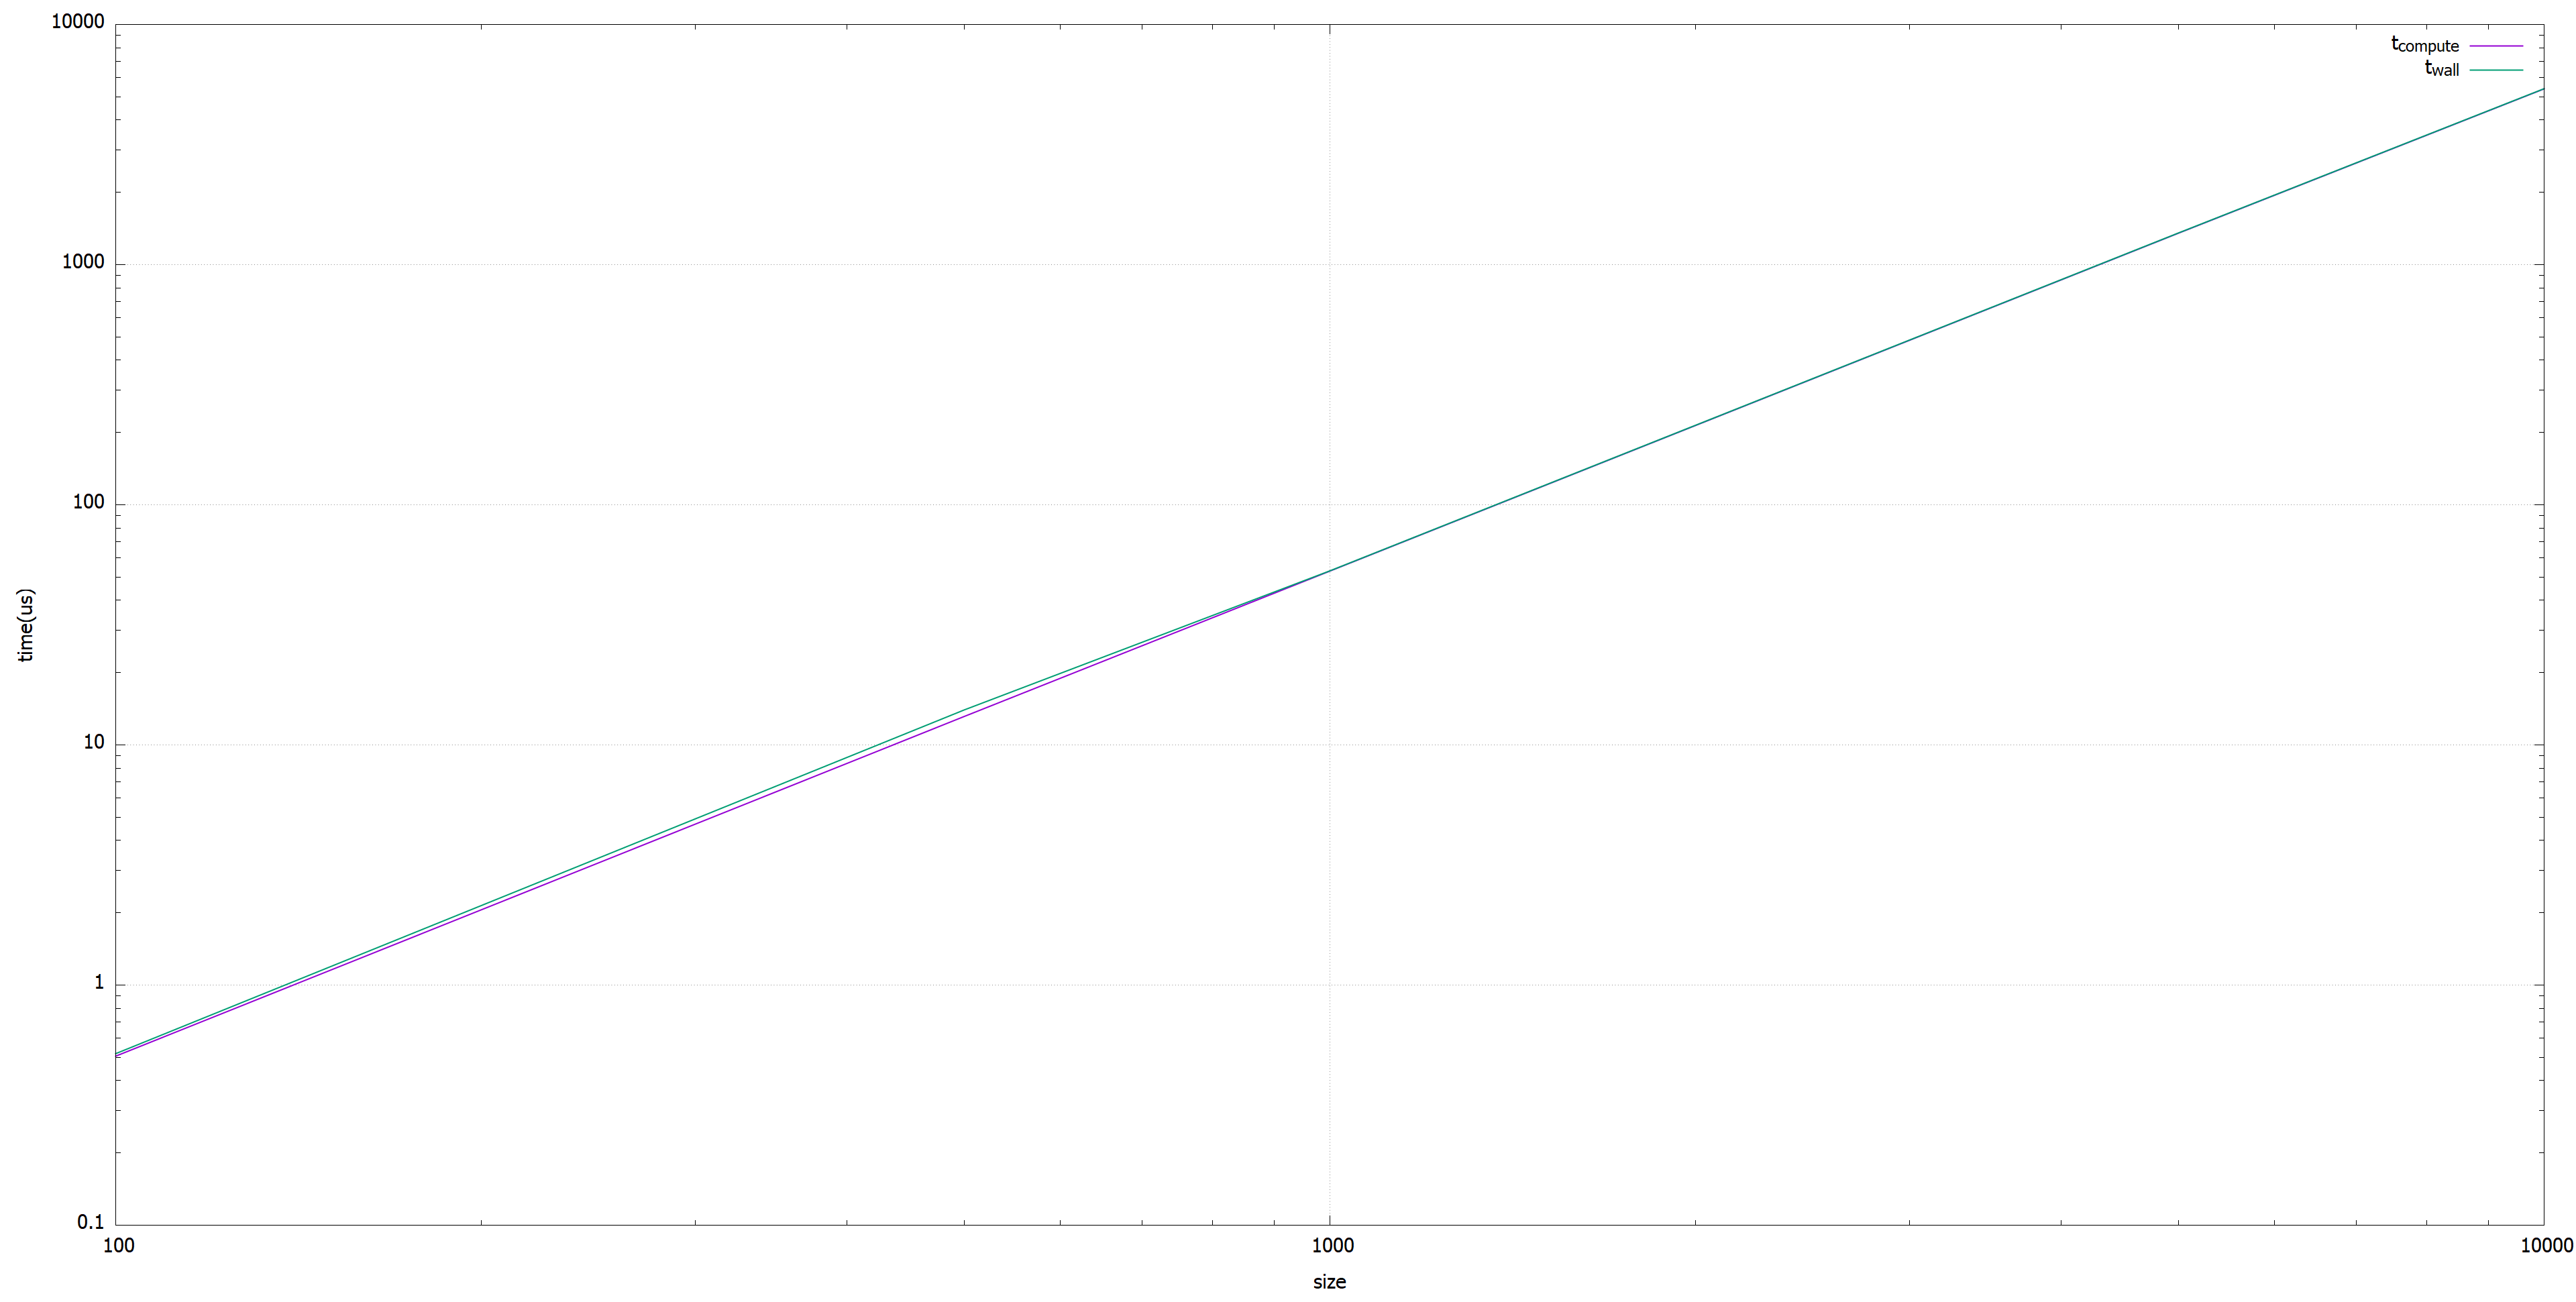
\includegraphics[width=0.9\linewidth]{../plot}
	\caption[$t_{compute,avg}$]{$t_{compute,avg}$}
	\label{fig:plot}
\end{figure}

\end{document}